\documentclass{article}
\usepackage{pdfpages}
\usepackage{graphicx}  % For PNG
\usepackage[left=2cm, right=2cm, top=2cm]{geometry}
\usepackage{minted}
% Give Table of Contents Hyperlinks
\usepackage{hyperref}
\hypersetup{
    colorlinks,
    citecolor=black,
    filecolor=black,
    linkcolor=black,
    urlcolor=blue
}
\pagenumbering{gobble}
% \pagenumbering{roman} % set the numbering style to lowercase letter

\title{\textbf{Homework 4}}

\author{MacMillan, Kyle}
\date{October 26, 2018}

\begin{document}


\addcontentsline{toc}{section}{Title}
\maketitle

\newpage
\tableofcontents
\addcontentsline{toc}{section}{Table of Contents}
\newpage
\listoffigures
\addcontentsline{toc}{section}{List of Figures}

\pagenumbering{roman}   % Set TOC page numbering to lowercase roman numerals


%%%%%%%%%%%%%%%%%%%%%%%%%%%% INTRO SECTION %%%%%%%%%%%%%%%%%%%%%%%%%%%%
\newpage
\hypersetup{
    colorlinks,
    citecolor=blue,
    filecolor=black,
    linkcolor=blue,
    urlcolor=blue
}
\pagenumbering{arabic}  % Set content page numbering to arabic numerals

\setcounter{page}{1}
\newpage
\section{\textbf{Problem 5.2}}
The meat and potatoes of this problem is in bump and gps callbacks, the 
rest is filler but can be found \href{https://github.com/macattackftw/RoboticsHW/blob/master/HW4/Problem2.py}{here}. The environment used is shown in Figure \ref{fig:stuck1}.

\begin{minted}{python}
def bumpCallback(self, msg):
    hit_obj = False
    for i in range(len(msg.data)):
        hit = unpack('b', msg.data[i])[0]
        if hit != 0:
            hit_obj = True

    if hit_obj:
        # Turn right
        self.bumps += 1
        self.setVel(0.0, 2.0)
    else:
        self.bumps = 0
        self.setVel(2.0, 2.0)


def gpsCallback(self, msg):
    # we need to move to goal if we are not bumping a wall
    if self.bumps == 0:
        # Wraps deals with the robot if it spins around somehow
        wraps = np.abs(int(msg.theta / (2 * np.pi)))
        theta = np.fabs(msg.theta) - (wraps * 2 * np.pi)
        beta = np.arctan2(self.goal[1] -
                          msg.y, self.goal[0] -
                          msg.x)
        k = 0.25
        alpha = beta - theta
        w1 = 2.0 + k * alpha
        w2 = 2.0 - k * alpha
        self.setVel(w1, w2)

\end{minted}

\begin{figure}[h]
    \centering
    
\includegraphics[pages=1]{stuck1}
    \caption{Problem 5.2 Stuck Robot}
    \label{fig:stuck1}
\end{figure}

\newpage
\section{\textbf{Problem 9}}
\subsection{Problem 9.1}
Figure \ref{fig:9.1} shows the required plot. The estimated robot location is:\\
$x = 882.079427083333$\\
$y = 443.766927083333$\\
$z = 521.18359375$\\

\begin{figure}[h]
    \centering
    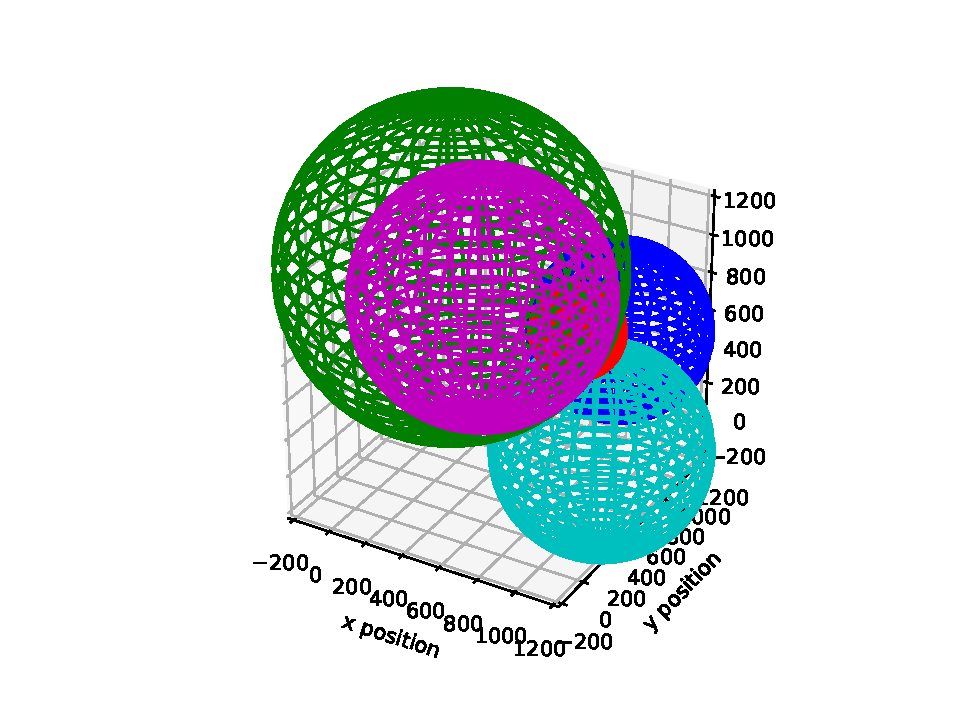
\includegraphics[pages=1]{problem9-1}
    \caption{Problem 9.1}
    \label{fig:9.1}
\end{figure}

This was obtained with a BFS octant descent. Each octant containing 
an intersection with all beacon radii is added to a queue to be processed. If 
an octant is processed it will be chopped up into 8 more octants and any of 
those subdivisions will be processed. After we have either hit maximum depth 
(capped at $2 * log_2(max\_length)$) or we fail to find an octant containing 
all beacon radii, the queue will empty. After the queue empties we find the 
maximum depth obtained and find all points that made it to that depth. The 
centroid of those points is the likely location of the robot. 

\newpage
\begin{minted}{python}
def findRobot(self):
    best_pts = []
    best_depth = []
    self.q.put(((self.a, self.b), 0))
    while not self.q.empty():
        pts, depth = self.q.get()
        self.checkGrids(pts, depth)
        best_pts.append(pts)
        best_depth.append(depth)

    centroid = Point()

    # Find the index that made it deepest and calculate the centroid
    idx = best_depth.index(max(best_depth))
    count = 0
    for i in range(len(best_depth)):
        if best_depth[i] == best_depth[idx]:
            centroid += best_pts[i][0].midpoint(best_pts[i][1])
            count += 1

    if centroid != Point(0, 0, 0):
        centroid.x = centroid.x / count
        centroid.y = centroid.y / count
        centroid.z = centroid.z / count

        self.robot_loc = centroid
        print('\nRobot at: {}'.format(str(self.robot_loc)))
    else:
        print('\nRobot not found!')
\end{minted}

\newpage
\begin{minted}{python}
def checkGrids(self, pts, depth):
    # For clarity:
    a = Point(pts[0].x, pts[0].y, pts[0].z)
    b = Point(pts[1].x, pts[1].y, pts[1].z)
    octants = 8

    grid = [0] * octants
    x_mid = ((b.x + a.x) / 2.0)
    y_mid = ((b.y + a.y) / 2.0)
    z_mid = ((b.z + a.z) / 2.0)
    ab_list = []

    # The 8 octants of pts a & b
    ab_list.append((a, Point(x_mid, y_mid, z_mid)))
    ab_list.append((Point(a.x, y_mid, a.z), Point(x_mid, b.y, z_mid)))
    ab_list.append((Point(x_mid, a.y, a.z), Point(b.x, y_mid, z_mid)))
    ab_list.append((Point(x_mid, y_mid, a.z), Point(b.x, b.y, z_mid)))

    ab_list.append((Point(a.x, a.y, z_mid), Point(x_mid, y_mid, b.z)))
    ab_list.append((Point(a.x, y_mid, z_mid), Point(x_mid, b.y, b.z)))
    ab_list.append((Point(x_mid, a.y, z_mid), Point(b.x, y_mid, b.z)))
    ab_list.append((Point(x_mid, y_mid, z_mid), b))

    # Fill grid with hits
    for b in self.beacons:
        # Check each block
        for i in range(octants):
            if b.onBlock(ab_list[i][0], ab_list[i][1]):
                grid[i] += 1
    found = 0
    for i in range(self.b_len):
        if grid[i] == self.b_len:
            found += 1

    if found == octants:
        return

    for i in range(octants):
        if grid[i] == self.b_len and depth < self.max_depth:
            self.q.put((ab_list[i], depth + 1))
\end{minted}


\newpage
\subsection{Problem 9.2}
\noindent $\lambda = c * 10 MHz$\\
$\lambda = 30\ meters$\\


Assuming phase shift $\theta = 10$ we can plug that into our formula to get

$$D' = L + \frac{\theta}{2\pi}\lambda$$
Therefore $D = \frac{D'}{2} = 0.833333333 + 15k$ where $k$ denotes an integer 
interval. We make the assumption that L is arbitrarily small compared to the 
distance travel and is therefore set to $0$. If the system has noise we will 
have to identify a range for $\frac{D'}{2}$, in this case it's $0.825\ to\ 
0.841666667 + 15k$. In order to differentiate between 20 and 250 meters we would 
need a second system at a $\lambda$ multiple that doesn't overlap before a 
distance of 250 meters.

\section{\textbf{Problem 10}}
\subsection{Problem 10.1}
\noindent$f = 0.8cm$\\
$b = 30cm$\\
$a = tan^-1 \big(\frac{z}{b-x}\big)$\\
$u = \frac{fx}{z}$\\

\noindent Given the above formulas we can say $a$ is in the range of: 
$45 < a < 90$ and for $u$: $3 < u < 45$.

\subsection{Probelm 10.2}
\noindent$e = 10\%$\\
$v_1 = 0.2cm$\\
$v_2 = 0.3cm$\\
$z = \frac{fb}{v_1 + v_2}$\\

\noindent Given the above formulas we can say that $f * b = 0.7 * 10 = 7$ but the range 
of z is dependent on $v_1 + v_2$, or:\\
$\frac{7}{0.18 + 0.27} <= z <= \frac{7}{0.22 + 0.33}$\\

\noindent With zero error we would expect $z = 14$, on the low end we expect $z = 12.72$ 
and on the upper end we expect $z = 15.56$, leaving an error of $3.7037\%$.
\end{document}
